193. \begin{figure}[ht!]
\center{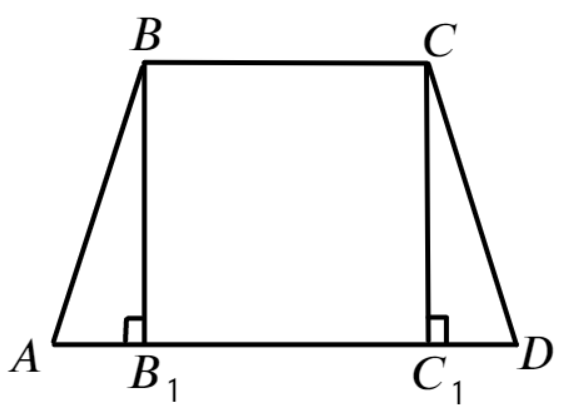
\includegraphics[scale=0.35]{g8-193.png}}
\end{figure}\\
Опустим высоты $BB_1$ и $CC_1.$ Так как трапеция равнобедренная, $AB_1=C_1D=(AD-BC):2=1,5.$ Найдём $\cos(\angle A)=\sqrt{1-\sin^2(\angle A)}=0,6.$ Тогда
$\cos(\angle A)=\cfrac{AB_1}{AB},\ 0,6=\cfrac{1,5}{AB},\ AB=\cfrac{5}{2}.$\\
